%----------------------------------------------------------------------------
\chapter{Gravitációs hatásából származó terhelés kompenzációja}
\label{sec:LatexTools}
%----------------------------------------------------------------------------

A bevezetőben illetve a szakdolgozatban elkészített telemanipulátor esetében is megfogalmaztam, hogy figyelembe vettem annak lehetőségét, hogy gravitációs hatásából származó terhelésre kompenzációs lehetőséget tervezzek. A tervezéshez korábban, egy típusú megoldást vettem figyelembe azonban ebben a fejezetben nagyon röviden a leggyakrabban előforduló lehetőségeket bemutatom. Ezt követően a megépített telemanipulátornál melyik megoldást fogom alkalmazni.

\section{Kompenzációs lehetőségek}
%----------------------------------------------------------------------------

Az elvégzett kutatásaim alapján a tömeg kompenzációs lehetőségeket két nagy csoportba sorolják, vannak az aktív illetve a passzív kompenzációs elven működő lehetőségek.

\begin{figure}[!h]
\centering
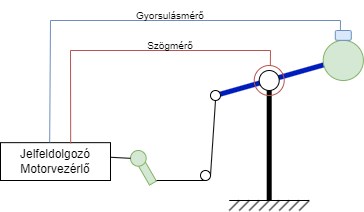
\includegraphics[width=70mm, keepaspectratio]{figures/Diagrammok/Kompenzacios_lehetosegek_aktiv}
\caption{Aktív kompenzációs lehetőségek szemléltetése}
\label{fig:Kompenzacios_lehetosegek_aktív}
\end{figure}

Az aktív rendszerek valamilyen szenzorral gyűjtött jel alapján aktuátorokkal valósítják meg a kompenzációt. A rendszer felépítésében összetett ugyanis szenzorból jelfeldolgozó rendszerből, teljesítmény elektronikából és valamilyen beavatkozó szervből kell felépíteni. Analógia alapján tekinthetjük, úgyhogy egy kis robot kell felépíteni. Ennek a kis robotnak pedig az a feladata, hogy az én esetemben a telemanipulátor karjin a gravitációs erő ne érződjön.


A passzív rendszerek pedig a fizika alaptörvényeit használják ki. Három kompenzációs erőt létrehozó elemből állhat, ezek pedig tömeg, rugó, vagy csillapító elem. Ezeknek a végtelen kombinációjával lehet találkozni a mérnöki életben. A következő ábrán egyszerűen ábrán bemutatom a legegyszerűbb és legelterjedtebb megoldásokat, amik alapján én is tovább haladtam.

\begin{figure}[!ht]
\centering
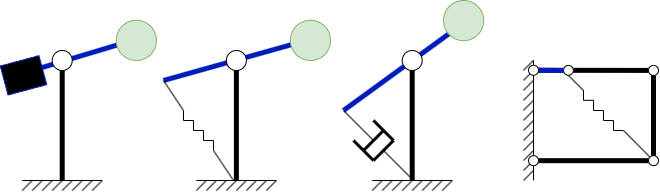
\includegraphics[width=125mm, keepaspectratio]{figures/Diagrammok/Kompenzacios_lehetosegek_passziv}
\caption{Passzív kompenzációs lehetőségek szemléltetése}
\label{fig:Kompenzacios_lehetosegek_passziv}
\end{figure}

Az első a tipikus ellensúlyos rendszer, amikor a csuklópontkörül kiegyensúlyozzuk a kar két oldalát. Eredményeképpen bármelyik állapotban megállítjuk a rendszer egyensúlyban van. A második egy rugós megoldás ez típusú kompenzáció a test stabil állapotának pozícióját változtatja meg. A stabil pont az lesz, ahol a rugó erő és a nehézségi erő egyensúlyba kerül. Harmadik megoldás egy csillapítóval egy ellenállást tesz a rendszerbe. Rezgéstanból megtanulva a csillapítási erő nagyobb, mint a nehézségi erő akkor a rendszer nyugalomban van, ha kisebb akkor a rendszer a különbség arányában a stabil pont irányába mozog. A negyedik megoldás egy szemléltetés, ebben az esetben összetettebb rendszer kinematikai kialakítását lehetséges úgy megadni, hogy a kinematikai elemek egymáshoz viszonyítottan tudják a kompenzációt létrehozni.

Fontos azonban megjegyezni, hogy a fent bemutatott megoldások tömegkompenzációs lehetőségek a nehézségi erőből fakadó kompenzációja sokkal összetettebb mechanikai rendszert igényel. A következő példán szemléltetem, hogy mi a tömeg kompenzáció és mi a nehézségi erő kompenzáció.

\begin{figure}[!ht]
\centering
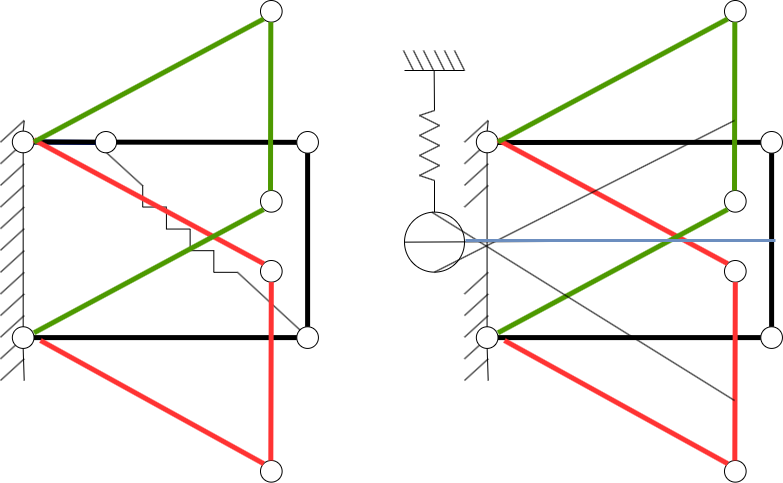
\includegraphics[width=125mm, keepaspectratio]{figures/Diagrammok/Tomeg_VS_Gravkomp}
\caption{Tömegkompenzációs és a nehézségi erő kompenzációjának szemléltetése}
\label{fig:Tomeg_VS_Gravkomp}
\end{figure}

A baloldali esetben a középső állásban van nyugalmi helyzetben a kinematika, a zöld  és a piros kitérítés esetében is vissza fog állni a stabil helyzetben. Itt a rugó megnyúlását használjuk fel. A jobboldali esetben viszont egy, olyan bonyolult mechanikai rendszer dolgozik, ahol a középső állapotban van a kék karnak a legnagyobb kompenzációs hatása a két szélső helyzetben a baloldalon található kényszer pályás idomnak köszönhetően ugyan olyan mértékben csökken a kompenzációs hatás. A második példában fontos kiemelni, hogy mindkét irányba csökken ez a hatás, míg az első példában az egyik irányba nő a másikba csökken.

\section{Telemanipulátoron alkalmazható kompenzáció}
%----------------------------------------------------------------------------

Az előzőekben bemutatott kutatási eredményeim alapján egyértelműen világos volt számomra milyen típusú kompenzációs megoldásokat kell figyelembe vennem a tervezés során.

A következő ábrán látható is milyen elrendezésben lenne a legegyszerűbb megvalósítani azt, hogy a telemanipulátort minél könnyebben lehessen használni. Az első feltételként azt támasztottam, hogy két parallelogramma kinematikai elrendezést építenék be. A későbbiekben számos előnyére kitérek, de jelen esetben a rugós és a ellensúlyos rendszer komplexen megvalósíthatóak lennének és nem kell minden egyes karon külön tervezni ezt a lehetőséget hanem egységes lenne. A másik nagyon előnye, hogy lehetőséget ad a prototípus gyártásra azaz kipróbálhatok többféle megoldást a későbbiekben.

\begin{figure}[!ht]
\centering
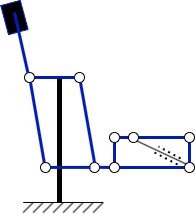
\includegraphics[width=55mm, keepaspectratio]{figures/Diagrammok/Megvalositott_kompenzacio}
\caption{Megvalósított kompenzációs rendszer}
\label{fig:Megvalositott_kompenzacio}
\end{figure}

%TODO ellensúly mérete

A diploma dolgozatom leadásának pillanatában az első paralelogrammás kinematikai rendszer ellensúlyos megoldással szereltem fel. A második paralelogrammás  kinematikai rendszerbe egy rugót helyeztem, ezzel a középső állapotba toltam a rendszer stabil pontját. A bonyolult kinematikai rendszert nem volt időm elkészíteni, de mindenképpen szeretném megvalósítani a későbbiekben.
